\subsection{Range Distribution Query}
\label{subsec:query}
%%
%%
The main goal of the pre-processing described so far is to improve the performance of arbitrary range distribution queries (run by the user or an application) on large-scale datasets. The pre-processing makes the query phase lightweight and fast. 

To answer a range distribution query for region $Q$, we first obtain the integral distribution - $H(Q_i)$ - at each corner point $Q_i$ of the query. To get $H(Q_i)$, we need to access and de-compress the codebook of the block that contains $Q_i$. We subdivide the range $[1,Q_i]$ into a set of sub-ranges denoted by $S(Q_i)= \{q_1,q_2, . . . ,q_\}$ using the algorithm described before. Distribution for each $q_i$ is retrieved from the codebook. The decoding phase also requires the set of template distributions $T$ to be loaded. However, since $T$ is a small set, compressing it is not mandatory.
%%
%%%%%%%%%%%%%%%%%%%
%% Diagram begins
%%%%%%%%%%%%%%%%%%%
\begin{figure}[!htb]
\centering
	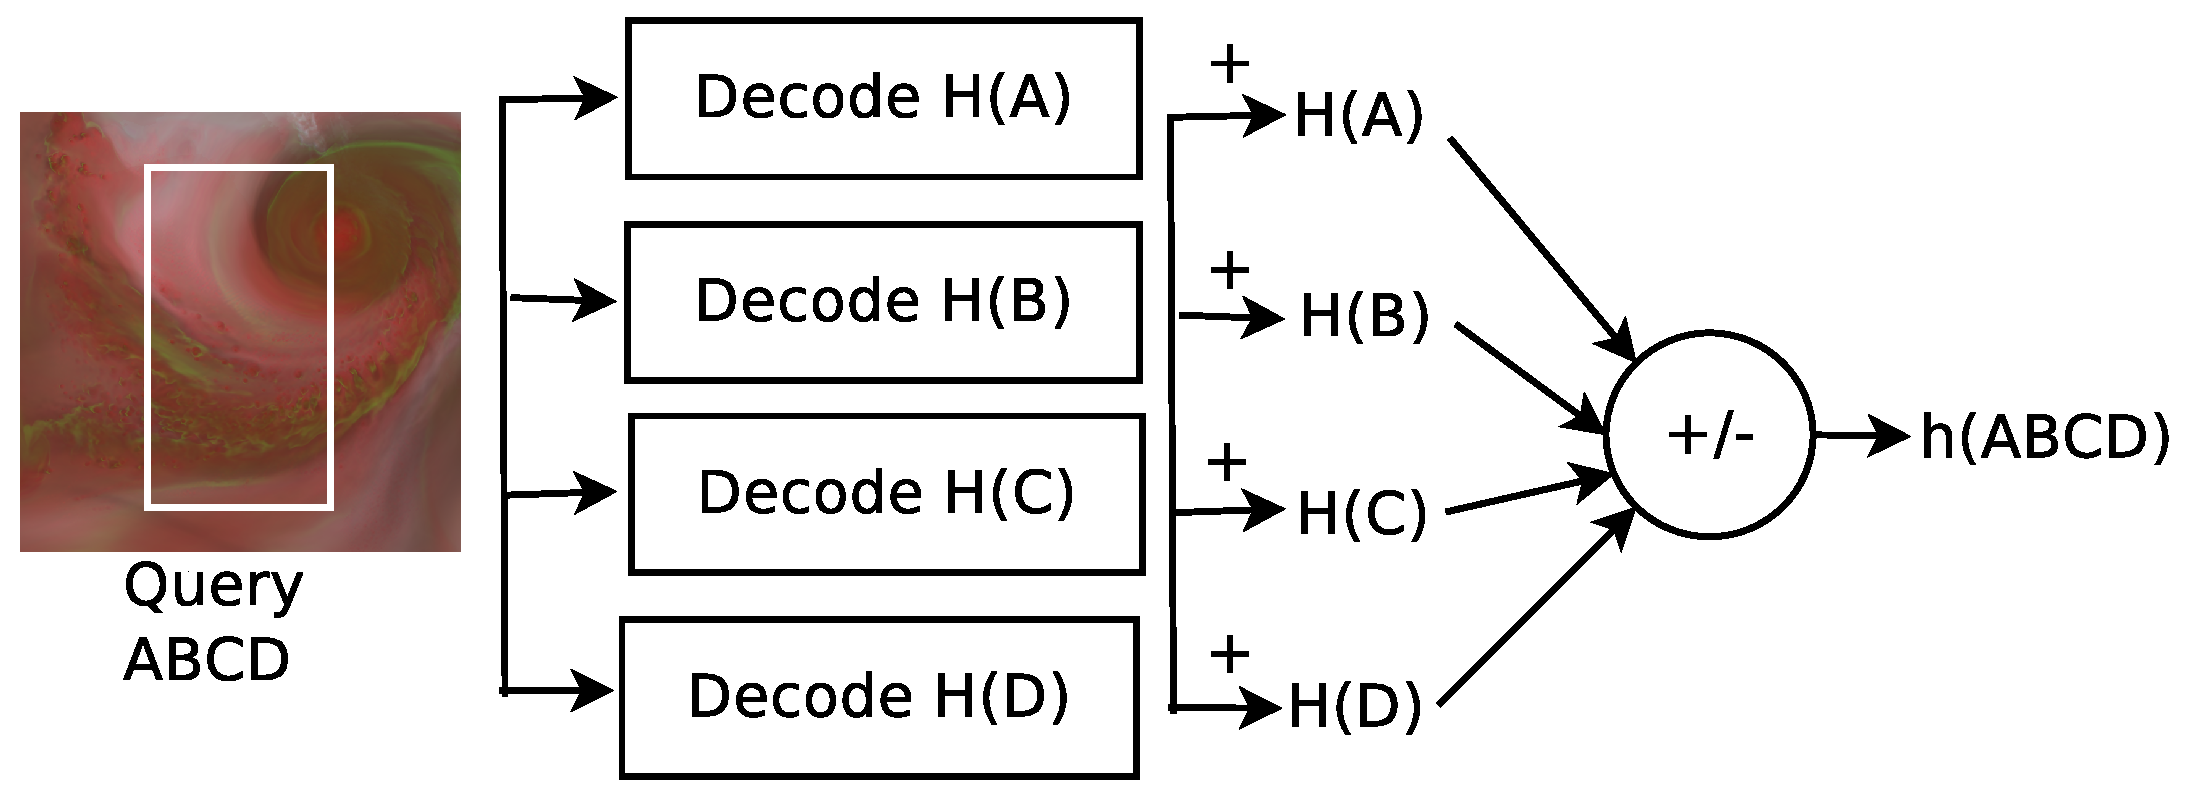
\includegraphics[width = 0.84\linewidth, keepaspectratio = true]{images/eps/decoding.eps}
	\caption{Retrieval of integral distribution at different locations requires to search the index tree up to different levels.}	
	\label{fig:retrieval}
\end{figure}
%%%%%%%%%%%%%%%%%%%
%% Diagram ends
%%%%%%%%%%%%%%%%%%%

Retrieval of a $h(q_j)$ from the codebook involves the following steps:
%%
\begin{packed_enumerate}
\item The codebook is used to retrieve the index to a template, say $k$ and a transformation $\tau$
\item Template histogram $h_k(T)$ is retrieved from template set $T$
\item The transformation is applied to the template histogram to obtain $\tau(h_k(T))$
\item The stored residuals $\delta$ for this mapping is retrieved, decompressed if needed, and applied to obtain $h(q_j) = \tau(h_k(T))+\delta$. 
\end{packed_enumerate}
%%
Addition of all $h(q_j)$s results in $H(Q_i)$, which eventually leads to $H(Q)$ (Figure~\ref{fig:retrieval}). 

Hence, our framework reduces the application workload in two ways. First, the query requires to access only eight corners, regardless of the query size. If the indexing results fit in memory, then it limits the memory access. If the indexing results for each data partition has been stored in compressed files, then it limits the number of disk accesses. Second, the retrieval of each corner distribution involves addition of a small number of spans, and then adding/subtracting corner histograms. Since the number of spans at any location $x$ is at most $\log x$, the computation required is much less compared to raw data scan, especially for large queries. Both of these lead to smaller query response time.
%%
%%
\remove
{
\subsection{Adaptations for Large Data}
\label{subsec:largedata}
%%
%%
%%%%%%%%%%%%%%%%%%%
%% Diagram begins
%%%%%%%%%%%%%%%%%%%
\begin{figure}[!htb]
\centering
	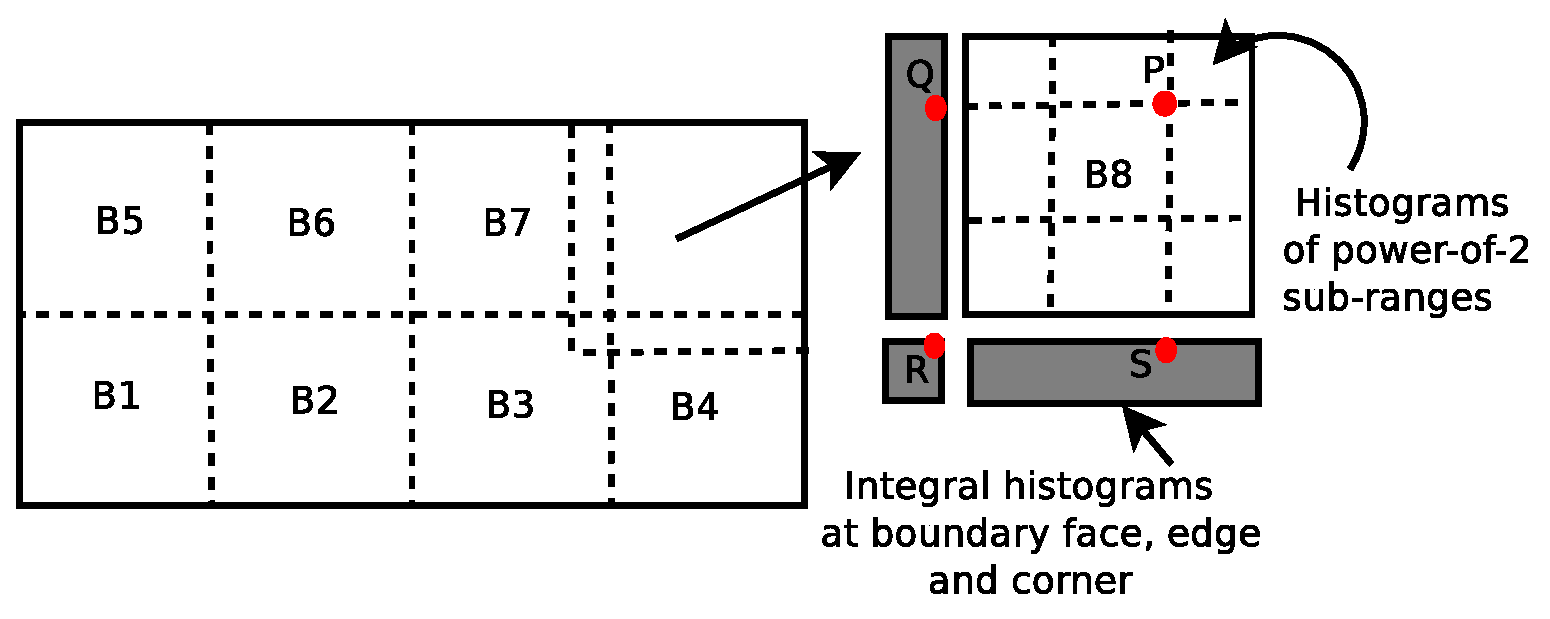
\includegraphics[width = 0.9\linewidth, keepaspectratio = true]{images/eps/ih_blockeddata.eps}
	\caption{Computing and encoding integral distributions from large data partitioned into blocks.}	
	\label{fig:blockeddata}
\end{figure}
%%%%%%%%%%%%%%%%%%%
%% Diagram ends
%%%%%%%%%%%%%%%%%%%
%%
%%
The benefit of such a framework is more clearly observed when the data is partitioned into blocks and distributed across many processors. In this section, we discuss a few adaptations which are necessary when applying this framework to partitioned data. 
%%
\begin{packed_itemize}
%%
\item Each data block simultaneously computes its own list of templates. A global list of templates is then created accumulating the local lists and the global list is distributed back to every block. A global list is used for indexing because even if two blocks are spatially far apart, they may contain similar distributions. 
\item Each data block is decomposed into power-of-two spans in its own local co-ordinates space. However, reconstructing these span distributions would not give back the global distribution of a corner point required for decoding. The global integral distribution at any point depends on its preceding blocks. Since speed is more important in the query phase, we pre-compute and store the integral distributions (in global coordinates space) for the corner point, three faces and three edges of the preceding blocks. Figure~\ref{fig:blockeddata} shows a 2D example where the integral distribution at point P in block B8 is computed from the spans and the pre-computed integral distributions at points Q, R and S.  
%%
\end{packed_itemize}
%%
}
 

